\chapter{Cubic functions}
\section{Defined on $\mdr$}
Let $f:\mdr \rightarrow \mdr, f(x) = a \cdot x^3 + b \cdot x^2 + c \cdot x + d$
be a cubic function with $a \in \mdr \setminus \Set{0}$ and
$b, c, d \in \mdr$.

\begin{figure}[htp]
    \centering
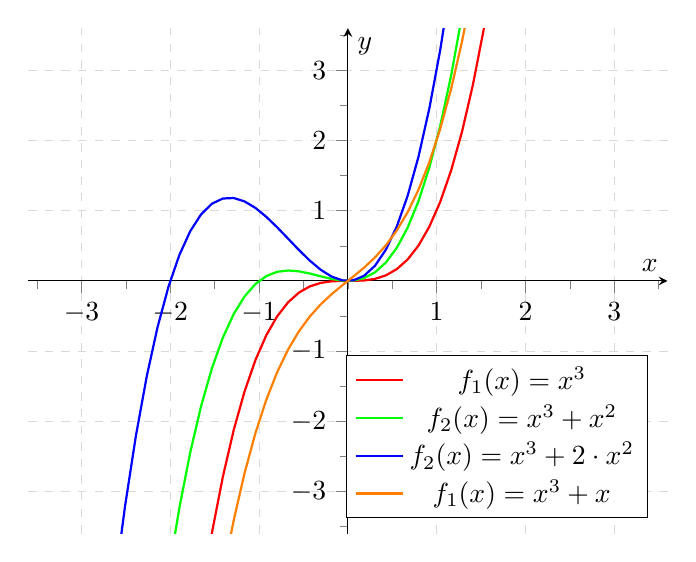
\begin{tikzpicture}
    \begin{axis}[
        legend pos=south east,
        axis x line=middle,
        axis y line=middle,
        grid = major,
        width=0.8\linewidth,
        height=8cm,
        grid style={dashed, gray!30},
        xmin=-3, % start the diagram at this x-coordinate
        xmax= 3, % end   the diagram at this x-coordinate
        ymin=-3, % start the diagram at this y-coordinate
        ymax= 3, % end   the diagram at this y-coordinate
        axis background/.style={fill=white},
        xlabel=$x$,
        ylabel=$y$,
        tick align=outside,
        minor tick num=-3,
        enlargelimits=true,
        tension=0.08]
      \addplot[domain=-3:3, thick,samples=50, red] {x*x*x};
      \addplot[domain=-3:3, thick,samples=50, green] {x*x*x+x*x};
      \addplot[domain=-3:3, thick,samples=50, blue] {x*x*x+2*x*x};
      \addplot[domain=-3:3, thick,samples=50, orange] {x*x*x+x};
      \addlegendentry{$f_1(x)=x^3$}
      \addlegendentry{$f_2(x)=x^3 + x^2$}
      \addlegendentry{$f_2(x)=x^3 + 2 \cdot x^2$}
      \addlegendentry{$f_1(x)=x^3 + x$}
    \end{axis}
\end{tikzpicture}
    \caption{Cubic functions}
\end{figure}

%
%\section{Special points}
%\todo[inline]{Write this}
%
%\section{Voronoi}
%
%For $b^2 \geq 3ac$
%
%\todo[inline]{Write this}

\subsection{Calculate points with minimal distance}
\begin{theorem}\label{thm:no-finite-solution}
    There cannot be a finite, closed form solution to the problem of finding
    a closest point $(x, f(x))$ to a given point $P$ when $f$ is
    a polynomial function of degree $3$ or higher.
\end{theorem}

\begin{proof}
    Suppose you could solve the closest point problem for arbitrary
    cubic functions $f = ax^3 + bx^2 + cx + d$ and arbitrary points $P = (x_P, y_P)$.

    Then you could solve the following problem for $x$:
    \begin{align}
        0  &\stackrel{!}{=} \left ((d_{P,f}(x))^2 \right )'\\
           &=-2 x_p + 2x -2y_p(f(x))' + (f(x)^2)'\\
           &= 2 f(x) \cdot f'(x) - 2 y_p f'(x) + 2x - 2 x_p\\
           &= f(x) \cdot f'(x) - y_p f'(x) + x - x_p\\
           &= \underbrace{f'(x) \cdot \left (f(x) - y_p \right )}_{\text{Polynomial of degree 5}} + x - x_p
    \end{align}

    General algebraic equations of degree 5 don't have a solution formula.\footnote{TODO: Quelle}
    Although here seems to be more structure, the resulting algebraic
    equation can be almost any polynomial of degree 5:\footnote{Thanks to Peter Košinár on \href{http://math.stackexchange.com/a/584814/6876}{math.stackexchange.com} for the idea.}

    \begin{align}
        0  &\stackrel{!}{=} f'(x) \cdot \left (f(x) - y_p \right ) + (x - x_p)\\
        &= \underbrace{3 a^2}_{= \tilde{a}} x^5 + \underbrace{5ab}_{= \tilde{b}}x^4 + \underbrace{2(2ac + b^2 )}_{= \tilde{c}}x^3 &+& \underbrace{3(ad+bc-ay_p)}_{= \tilde{d}} x^2 \\
        & &+& \underbrace{(2 b d+c^2+1-2 b y_p)}_{= \tilde{e}}x+\underbrace{c d-c y_p-x_p}_{= \tilde{f}}\\
        0 &\stackrel{!}{=} \tilde{a}x^5 + \tilde{b}x^4 + \tilde{c}x^3 + \tilde{d}x^2 + \tilde{e}x + \tilde{f}
    \end{align}

    \begin{enumerate}
        \item For any coefficient $\tilde{a} \in \mdr_{> 0}$ of $x^5$ we can choose $a := \frac{1}{3} \sqrt{\tilde{a}}$ such that we get $\tilde{a}$.
        \item For any coefficient $\tilde{b} \in \mdr \setminus \Set{0}$ of $x^4$ we can choose $b := \frac{1}{5a} \cdot \tilde{b}$ such that we get $\tilde{b}$.
        \item With $c := -2b^2 + \frac{1}{4a} \tilde{c}$, we can get any value of $\tilde{c} \in \mdr$.
        \item With $d := -bc + a y_p + \frac{1}{a} \tilde{d}$, we can get any value of $\tilde{d} \in \mdr$.
        \item With $y_p := \frac{1}{2b}(2bd + c^2)\cdot \tilde{e}$, we can get any value of $\tilde{e} \in \mdr$.
        \item With $x_p := cd - c y_P+\tilde{f}$, we can get any value of $\tilde{f} \in \mdr$.
    \end{enumerate}

    The first restriction guaratees that we have a polynomial of
    degree 5. The second one is necessary, to get a high range of
    $\tilde{e}$.

    This means that there is no finite solution formula for the problem of
    finding the closest points on a cubic function to a given point,
    because if there was one, you could use this formula for finding
    roots of polynomials of degree 5. $\qed$
\end{proof}


\subsection{Another approach}
Just like we moved the function $f$ and the point to get in a
nicer situation, we can apply this approach for cubic functions.

\begin{figure}[htp]
    \centering
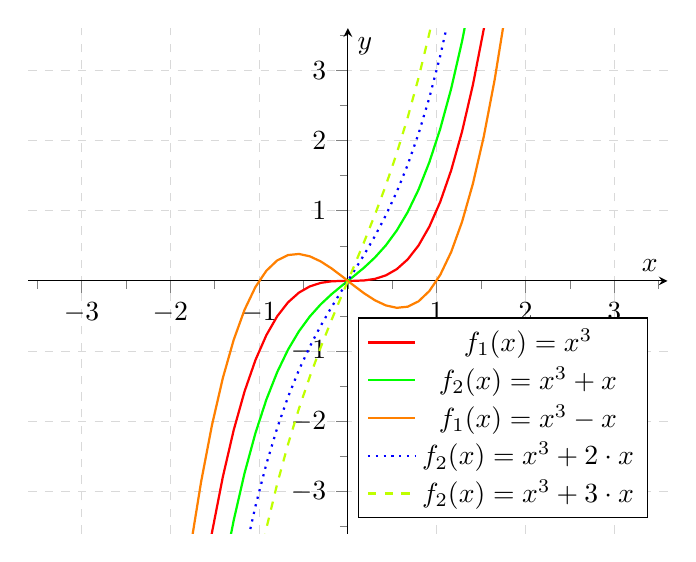
\begin{tikzpicture}
    \begin{axis}[
        legend pos=south east,
        axis x line=middle,
        axis y line=middle,
        grid = major,
        width=0.8\linewidth,
        height=8cm,
        grid style={dashed, gray!30},
        xmin=-3, % start the diagram at this x-coordinate
        xmax= 3, % end   the diagram at this x-coordinate
        ymin=-3, % start the diagram at this y-coordinate
        ymax= 3, % end   the diagram at this y-coordinate
        axis background/.style={fill=white},
        xlabel=$x$,
        ylabel=$y$,
        tick align=outside,
        minor tick num=-3,
        enlargelimits=true,
        tension=0.08]
      \addplot[domain=-3:3, thick,samples=50, red] {x*x*x};
      \addplot[domain=-3:3, thick,samples=50, green] {x*x*x+x};
      \addplot[domain=-3:3, thick,samples=50, orange] {x*x*x-x};
      \addplot[domain=-3:3, thick,samples=50, blue, dotted] {x*x*x+2*x};
      \addplot[domain=-3:3, thick,samples=50, lime, dashed] {x*x*x+3*x};
      \addlegendentry{$f_1(x)=x^3$}
      \addlegendentry{$f_2(x)=x^3 + x$}
      \addlegendentry{$f_1(x)=x^3 - x$}
      \addlegendentry{$f_2(x)=x^3 + 2 \cdot x$}
      \addlegendentry{$f_2(x)=x^3 + 3 \cdot x$}
    \end{axis}
\end{tikzpicture}
    \caption{Cubic functions with $b = d = 0$}
\end{figure}

First, we move $f_0$ by $\frac{b}{3a}$ in $x$ direction, so

\[f_1(x) = ax^3 + \frac{b^2 (c-1)}{3a} x + \frac{2b^3}{27 a^2} - \frac{bc}{3a} + d \;\;\;\text{ and }\;\;\;P_1 = (x_P + \frac{b}{3a}, y_P)\]

because

\begin{align}
    f_1(x) &= a \left (x - \frac{b}{3a} \right )^3 + b \left (x-\frac{b}{3a} \right )^2 + c \left (x-\frac{b}{3a} \right ) + d\\
           &= a \left (x^3 - 3 \frac{b}{3a}x^2 + 3 (\frac{b}{3a})^2 x - \frac{b^3}{27a^3} \right )
             +b \left (x^2 - \frac{2b}{3a} x + \frac{b^2}{9a^2} \right )
             +c x - \frac{bc}{3a} + d\\
            &= ax^3 - bx^2 + \frac{b^2}{3a}x - \frac{b^3}{27 a^2}\\
            & \;\;\;\;\;\;+ bx^2 - \frac{2b^2}{3a}x + \frac{b^3}{9a^2}\\
            & \;\;\;\;\;\;\;\;\;\;\;\; + c x - \frac{bc}{3a} + d\\
            &= ax^3 + \frac{b^2}{3a}\left (1-2+c \right )x + \frac{b^3}{9a^2} \left (1-\frac{1}{3} \right )- \frac{bc}{3a} + d
\end{align}

The we move it in $y$ direction by $- (\frac{2b^3}{27 a^2} - \frac{bc}{3a} + d)$:

\[f_2(x) = ax^3 + \frac{b^2 (c-1)}{3a} x \;\;\;\text{ and }\;\;\;P_2 = (x_P + \frac{b}{3a}, y_P - (\frac{2b^3}{27 a^2} - \frac{bc}{3a} + d))\]

Multiply everything by $\sgn(a)$:

\[f_3(x) = \underbrace{|a|}_{=: \alpha}x^3 + \underbrace{\frac{b^2 (c-1)}{3|a|}}_{=: \beta} x \;\;\;\text{ and }\;\;\;P_2 = (x_P + \frac{b}{3a}, \sgn(a) (y_P - \frac{2b^3}{27 a^2} + \frac{bc}{3a} - d))\]

Now the problem seems to be much simpler. The function $\alpha x^3 + \beta x$
with $\alpha > 0$ is centrally symmetric to $(0, 0)$.

\todo[inline]{Und weiter?}

\subsection{Number of points with minimal distance}
As this leads to a polynomial of degree 5 of which we have to find
roots, there cannot be more than 5 solutions.
\todo[inline]{Can there be 3, 4 or even 5 solutions? Examples!

After looking at function graphs of cubic functions, I'm pretty
sure that there cannot be 4 or 5 solutions, no matter how you
chose the cubic function $f$ and $P$.

I'm also pretty sure that there is no polynomial (no matter what degree)
that has more than 3 solutions.}


\subsection{Interpolation and approximation}
\subsubsection{Quadratic spline interpolation}
You could interpolate the cubic function by a quadratic spline.

\subsubsection{Bisection method}
\todo[inline]{TODO}

\subsubsection{Newtons method}
One way to find roots of functions is Newtons method. It gives an
iterative computation procedure that can converge quadratically
if some conditions are met:

\begin{theorem}[local quadratic convergence of Newton's method\footnotemark]
    Let $D \subseteq \mdr^n$ be open and $f: D \rightarrow \mdr^n \in C^2(\mdr)$.
    Let $x^* \in D$ with $f(x^*) = 0$ and the Jaccobi-Matrix $f'(x^*)$
    should not be invertable when evaluated at the root.

    Then there is a sphere
    \[K := K_\rho(x^*) = \Set{x \in \mdr^n | \|x- x^*\|_\infty \leq \rho} \subseteq D\]
    such that $x^*$ is the only root of $f$ in $K$. Furthermore,
    the elements of the sequence
    \[ x_{n+1} = x_n - \frac{f'(x_n)}{f(x_n)}\]
    are for every starting value $x_0 \in K$ again in $K$ and
    \[\lim_{n \rightarrow \infty} x_k = x^*\]
    Also, there is a constant $C > 0$ such that
    \[\|x^* - x_{n+1} \| = C \|x^* - x_n\|^2 \text{ for } n \in \mathbb{N}_0\|\]
\end{theorem}
\footnotetext{Translated from German to English from lecture notes of "Numerische Mathematik für die Fachrichtung Informatik
und Ingenieurwesen" by Dr. Weiß, KIT}

The approach is extraordinary simple. You choose a starting value
$x_0$ and compute

\[x_{n+1} = x_n - \frac{f(x_n)}{f'(x_n)}\]

As soon as the values don't change much, you are close to a root.
The problem of this approach is choosing a starting value that is
close enough to the root. So we have to have a \enquote{good}
initial guess.
\clearpage

\subsubsection{Muller's method}
Muller's method was first presented by David E. Muller in 1956.

\todo[inline]{Paper? Might this be worth a try?}

\subsubsection{Bisection method}
The idea of the bisection method is the following:

Suppose you know a finite intervall $[a,b]$ in which you have
exactly one root $r \in (a,b)$ with $f(r) = 0$.

Then you can half that interval:
    \[[a, b] = \left [a, \frac{a+b}{2} \right ] \cup \left [\frac{a+b}{2}, b \right ]\]

Now three cases can occur:
\begin{enumerate}
    \item[Case 1] $f(\frac{a+b}{2})=0$: You have found the exact root.
    \item[Case 2] $\sgn(a) = \sgn(\frac{a+b}{2})$: Continue searching in $[\frac{a+b}{2}, b]$
    \item[Case 3] $\sgn(b) = \sgn(\frac{a+b}{2})$: Continue searching in $[a, \frac{a+b}{2}]$
\end{enumerate}

\todo[inline]{Which intervall can I choose? How would I know that there is exactly one root?}

\subsubsection{Bairstow's method}
Cite from Wikipedia:
The algorithm first appeared in the appendix of the 1920 book "Applied Aerodynamics" by Leonard Bairstow. The algorithm finds the roots in complex conjugate pairs using only real arithmetic.

[...]
\todo[inline]{Find a source for the following!}
A particular kind of instability is observed when the polynomial has odd degree and only one real root.



\section{Defined on a closed interval $[a,b] \subseteq \mdr$}
The point with minimum distance can be found by:
\[\underset{x\in[a,b]}{\arg \min d_{P,f}(x)} = \begin{cases}
 S_3(f, P) &\text{if } S_3(f, P) \cap [a,b] \neq \emptyset\\
  TODO     &\text{if } S_3(f, P) \cap [a,b] = \emptyset
    \end{cases}\]
